\documentclass[12pt,a4paper]{report}
\pagestyle{plain}

\usepackage{geometry}
\geometry{a4paper,scale=0.8}
\usepackage{color}
\usepackage{extarrows}
\usepackage{bm}
\usepackage{graphicx}

\renewcommand\thesection{Part \arabic{section}}
\renewcommand\thesubsection{\arabic{section}.\arabic {subsection}}
\newcommand{\tablecell}[1]{\begin{tabular}{@{}c@{}}#1\end{tabular}}  

\usepackage{array}
\newcommand{\PreserveBackslash}[1]{\let\temp=\\#1\let\\=\temp}
\newcolumntype{C}[1]{>{\PreserveBackslash\centering}p{#1}}

\title{Department of Informatics,\\ King's College London\\
Data Mining(7CCSMDM1)\\ Answer of Assignment 1}
\author{Jinlai Ning}

\begin{document}\large
	\maketitle
	\section{Classification}
	\subsection{}
	\begin{tabular}{|c|c|}
	\hline
 	Number of instances&48842\\
  	Number of missing values&6465\\
  	Fraction of missing values over all attribute values&0.95\%\\
  	Number of instances with missing value&3620\\
  	Fraction of instances with missing values over all instances&7.41\%\\
	\hline
	\end{tabular}
	\subsection{}
	\begin{tabular}{|c|C{13cm}|}
	\hline
	Attributes&Encoded value\\
	\hline
  	age&[2 3 1 0 4]\\
	workclass&[7 6 4 1 2 0 5 8 3]\\
   	education&[ 9 11  1 12  6 15  7  8  5 10 14  4  0  3 13  2]\\
   	education-num&[12  8  6 13  4  9 11 10  3 15 14  2  5  1  0  7]\\
   	marital-status&[4 2 0 3 5 1 6]\\
   	occupation&[ 1  4  6 10  8 12  3 14  5  7 13  0 11  2  9]\\
   	relationship&[1 0 5 3 4 2]\\
   	race&[4 2 1 0 3]\\
   	sex&[1 0]\\
   	capitalgain&[1 0 4 2 3]\\
   	capitalloss&[0 3 1 2 4]\\
   	hoursperweek&[2 0 3 4 1]\\
   	native-country&[39  5 23 19  0 26 35 33 16  9  2 11 20 30 22 31  4  1 37  7 25 36 14 32
  6  8 10 13  3 24 41 29 28 34 38 12 27 40 17 21 18 15]\\
	\hline
	\end{tabular}
	\subsection{}
  	Error rate when just ignoring instances with missing values: 17.26\%.
	\subsection{}
	Both decision tree are tested based on the same test set split from D.\\
  	Error rate when building decision tree with D1: 18.03\%.\\
  	Error rate when building decision tree with D2: 8.34\%.\\
  	It is clear that error rate is lower when building decision tree based on D2. It suggests that filling missing values with most common value performs better than just giving missing value a new value 'missing value'.
	\section{Clustrering}
	\subsection{}
	\begin{tabular}{|c|c|c|}
	\hline
	j&$\mu=\sum_{i=1}^{m}x_{i,j}$&$\left[x_{j,min},x_{j,max}\right]$\\
	\hline
	Fresh&12000.30&[3,112151]\\
	Milk&5796.27&[55,73498]\\
	Grocery&7951.28&[3,92780]\\
	Frozen&3071.93&[25,60896]\\
	Detergents\_Paper&2881.49&[3,40827]\\
	Delicassen&1524.87&[3,47943]\\
	\hline
	\end{tabular}

	\subsection{}
	\begin{figure}[htbp]
	\centering 
	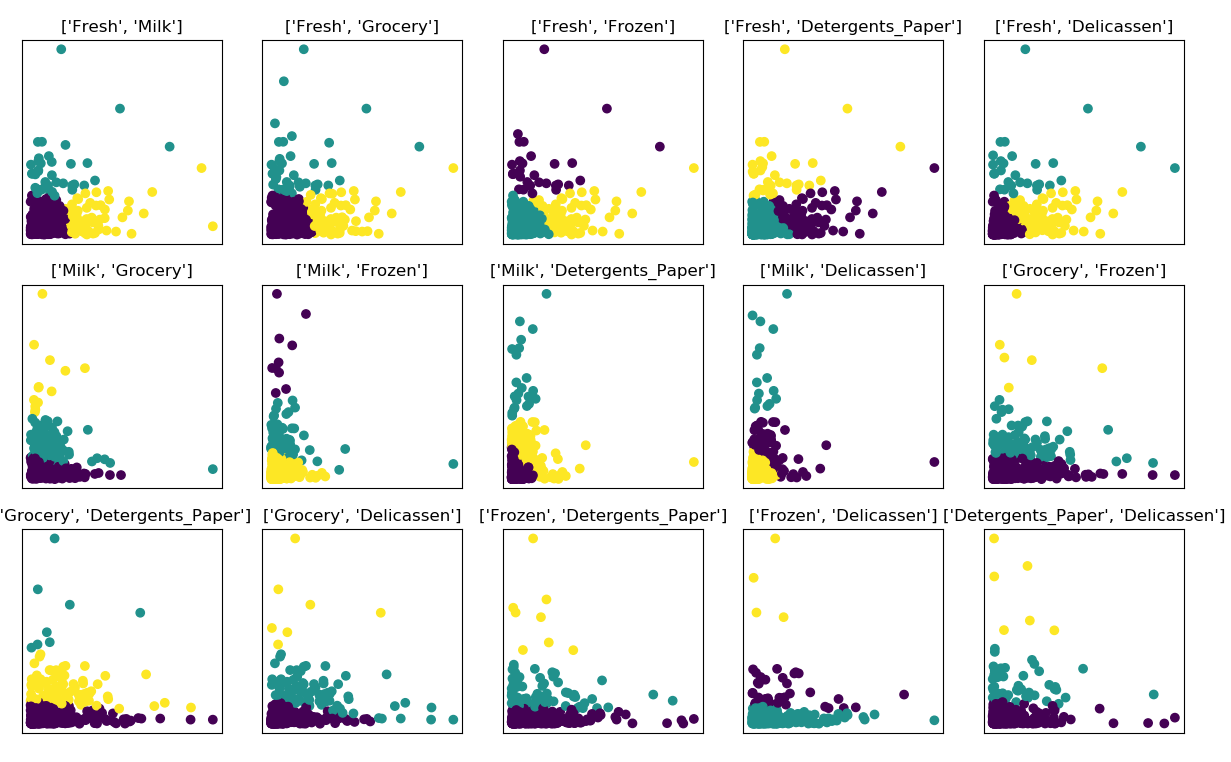
\includegraphics[width=\textwidth]{kmeans_15.png} 
	%\caption{Results of kmeans}  
	\end{figure}
	
	\subsection{}
	\resizebox{0.75\textwidth}{!}{
	\begin{tabular}{|c|c|c|c|}
	\hline
	&k=3&k=5&k=10\\
	\hline
	BC&3.1820$e^{+09}$&2.7368$e^{+10}$&1.7359$e^{+11}$\\
	WC&8.0333$e^{+10}$&5.3106$e^{+10}$&3.0377$e^{+10}$\\
	BC/WC&0.039610&0.515350&5.714309\\
	\hline
	\end{tabular}}\\ 
	
	\noindent It is clear that the BC/WC is the biggest when k=10, followed by k=5 and is the lowest when k=3. It suggests that 10 clusters are more suitable than 5 and 3 for clustering the wholesale customers data set. 
\end{document}